\begin{topic}{young-diagram}{Young diagram}
    Given a partition $\lambda = (\lambda_1, \lambda_2, \ldots, \lambda_k)$ of a non-negative integer $n \ge 0$, a \textbf{Young diagram} of shape $\lambda$ is a collection of $n$ boxes, arranged in left-aligned rows, such that row $i$ has $\lambda_i$ boxes. For example, a Young diagram of shape $(5, 3, 2)$ is given by:
    \[ 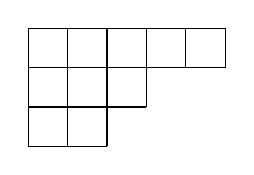
\begin{tikzpicture}
        \begin{scope}[scale=0.5]
            \draw (0, 3) -- (5, 3); \draw (0, 2) -- (5, 2); \draw (0, 1) -- (3, 1); \draw (0, 0) -- (2, 0); \draw (0, 3) -- (0, 0); \draw (1, 3) -- (1, 0); \draw (2, 3) -- (2, 0); \draw (3, 3) -- (3, 1); \draw (4, 3) -- (4, 2); \draw (5, 3) -- (5, 2);
        \end{scope}
    \end{tikzpicture} \]
    The \textit{arm length} of a box $s$, denoted $a_\lambda(s)$, is the number of boxes to the right of $s$. The \textit{leg length} of $s$, denoted $l_\lambda(s)$, is the number of boxes below $s$.
    
    A \textbf{Young tableau} is obtained from a Young diagram by filling in the boxes with numbers. A Young tableau is \textbf{standard} if the entries in each row and each column are increasing.
\end{topic}

\begin{topic}{generating-function}{generating function}
    The \textbf{generating function} of a sequence $a_0, a_1, a_2, \ldots$ in a \tref{AA:ring}{commutative ring} $R$ is the formal power series
    \[ \sum_{n = 0}^{\infty} a_n t^n = a_0 + a_1 t + a_2 t^2 + \cdots \in R \llbracket t \rrbracket . \]
\end{topic}

\begin{example}{generating-function}
    \begin{itemize}
        \item The generating function of the constant sequence $1, 1, 1, \ldots$ is
        \[ \sum_{n = 0}^{\infty} t^n = \frac{1}{1 - t} . \]
        \item The generating function of the linear sequence $0, 1, 2, 3, \ldots$ is
        \[ \sum_{n = 0}^{\infty} n t^{n} = t \cdot \frac{d}{dt} \sum_{n = 0}^{\infty} t^{n} = t \cdot \frac{d}{dt} \left( \frac{1}{1 - t} \right) = \frac{t}{(1 - t)^2} . \]
        \item The generating function of 
    \end{itemize}
\end{example}

\begin{example}{generating-function}
    Assuming $R$ has \tref{AA:characteristic}{characteristic} zero, the sequence can be obtained from the generating function $F \in R \llbracket t \rrbracket$ as follows. Writing
    \[ F = \sum_{n = 0}^{\infty} a_n t^n = a_0 + a_1 t + a_2 t^2 + \cdots , \]
    we obtain the coefficients $a_n$ from the $n$-th derivatives of $F$ as
    \[ a_n = \frac{F^{(n)}(0)}{n!} . \]
\end{example}

\begin{topic}{mobius-function}{Möbius function}
    The \textbf{Möbius function} $\mu$ is the function that assigns to any positive integer $n > 0$ the value
    \[ \mu(n) = \sum_{\substack{1 \le k \le n \\ \gcd(k, n) = 1}} e^{2\pi i \frac{k}{n}} , \]
    or alternatively,
    \[ \mu(n) = \left\{ \begin{array}{cl}
         +1 & \textup{ if $n$ is square-free with even number of prime factors}, \\
         -1 & \textup{ if $n$ is square-free with odd number of prime factors}, \\
         0 & \textup{ if $n$ has a squared prime factor}.
    \end{array} \right. \]
\end{topic}

\begin{example}{mobius-function}
    The first few values of $\mu$ are given by
    \[ \begin{array}{lllll}
        \mu(1) = 1, & \mu(2) = -1, & \mu(3) = -1, & \mu(4) = 0, & \mu(5) = -1, \\
        \mu(6) = 1, & \mu(7) = -1, & \mu(8) = 0, & \mu(9) = 0, & \mu(10) = 1, \ldots
    \end{array} \]
\end{example}